% Cute front-facing bear plush -- standalone TikZ (xelatex ready)
\documentclass[tikz,border=0pt]{standalone}

\definecolor{bgWarm}{RGB}{255,247,236}
\definecolor{bgAccent}{RGB}{253,234,208}
\definecolor{bgAccentB}{RGB}{250,224,196}
\definecolor{furMain}{RGB}{216,167,113}
\definecolor{furDark}{RGB}{178,126,76}
\definecolor{furMid}{RGB}{200,148,96}
\definecolor{furLight}{RGB}{243,219,181}
\definecolor{furCream}{RGB}{250,236,211}
\definecolor{padPink}{RGB}{234,176,152}
\definecolor{padDeep}{RGB}{216,146,124}
\definecolor{inkBrown}{RGB}{82,50,36}
\definecolor{blushPink}{RGB}{240,161,150}
\definecolor{badgeRed}{RGB}{224,106,99}
\definecolor{shadowWarm}{RGB}{238,220,198}

\begin{document}
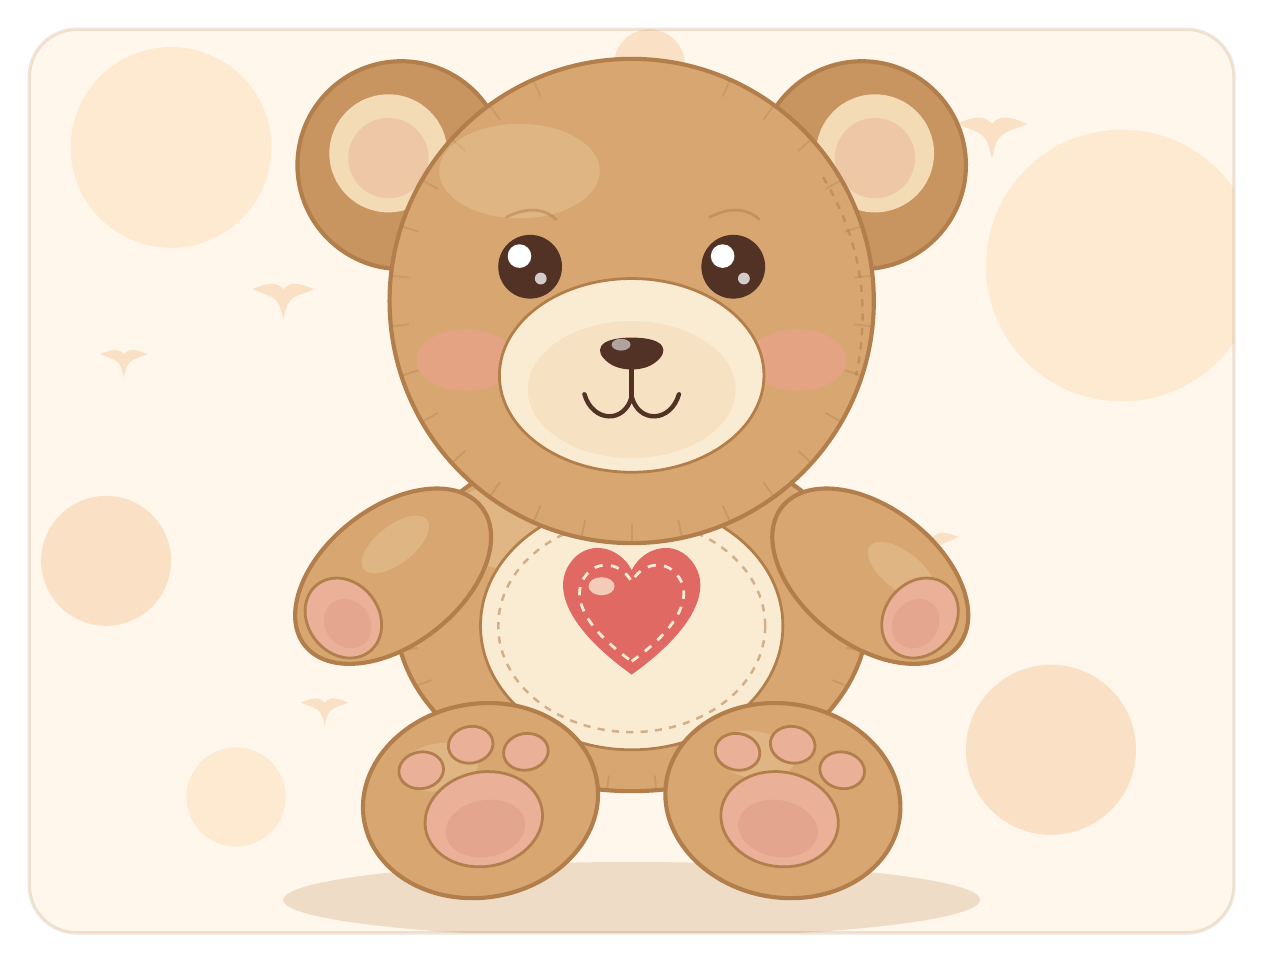
\begin{tikzpicture}[
  scale=1.5,
  outline/.style={draw=furDark, line width=1.5pt, line join=round},
  thinline/.style={draw=furDark, line width=1.0pt},
  stitch/.style={draw=furDark, line width=0.9pt, dash pattern=on 2.6pt off 2.6pt, opacity=0.55}
]

% ---------------------------------------------------------------- background
\fill[bgWarm, rounded corners=0.6cm] (-5.1,-4.3) rectangle (5.1,3.35);
\begin{scope}
\clip[rounded corners=0.6cm] (-5.1,-4.3) rectangle (5.1,3.35);

\fill[bgAccent] (-3.9,2.35) circle (0.85);
\fill[bgAccent] (4.15,1.35) circle (1.15);
\fill[bgAccentB] (-4.45,-1.15) circle (0.55);
\fill[bgAccentB] (3.55,-2.75) circle (0.72);
\fill[bgAccent] (-3.35,-3.15) circle (0.42);
\fill[bgAccentB] (0.15,3.05) circle (0.30);

% small four-point sparkles
\foreach \sx/\sy/\sr in {-2.95/1.15/0.26, 3.05/2.55/0.30, -4.30/0.60/0.20, 2.55/-0.95/0.22, -2.60/-2.35/0.20}{
  \fill[bgAccentB] (\sx,\sy)
    .. controls ({\sx+0.16*\sr},{\sy+0.16*\sr}) and ({\sx+0.32*\sr},{\sy+0.30*\sr}) .. ({\sx+\sr},\sy)
    .. controls ({\sx+0.32*\sr},{\sy-0.30*\sr}) and ({\sx+0.16*\sr},{\sy-0.16*\sr}) .. (\sx,{\sy-\sr})
    .. controls ({\sx-0.16*\sr},{\sy-0.16*\sr}) and ({\sx-0.32*\sr},{\sy-0.30*\sr}) .. ({\sx-\sr},\sy)
    .. controls ({\sx-0.32*\sr},{\sy+0.30*\sr}) and ({\sx-0.16*\sr},{\sy+0.16*\sr}) .. cycle;
}

% ------------------------------------------------------------- ground shadow
\fill[shadowWarm] (0,-4.02) ellipse (2.95 and 0.32);

% ---------------------------------------------------------------------- ears
\foreach \s in {-1,1}{
  \fill[furMid, outline] ({\s*1.95},2.20) circle (0.88);
  \fill[furLight] ({\s*2.06},2.30) circle (0.50);
  \fill[padPink, opacity=0.45] ({\s*2.06},2.26) circle (0.34);
}

% ---------------------------------------------------------------------- body
\fill[furMain, outline] (0,-1.60) ellipse (2.00 and 1.50);

% fur ticks around the body silhouette
\foreach \a in {0,12,...,348}{
  \draw[furDark, line width=0.7pt, opacity=0.35, line cap=round]
    ({2.00*cos(\a)},{-1.60+1.50*sin(\a)}) -- ({1.86*cos(\a)},{-1.60+1.38*sin(\a)});
}

% soft sheen on the stuffing
\fill[furLight, opacity=0.30] (-0.95,-0.85) ellipse (0.62 and 0.38);

% belly patch (smoother, lighter texture)
\fill[furCream, thinline] (0,-1.70) ellipse (1.28 and 1.05);
\draw[stitch] (0,-1.70) ellipse (1.13 and 0.90);

% ------------------------------------------------------------- chest badge
\begin{scope}[shift={(0,-1.45)}, scale=0.85]
  \fill[badgeRed]
      (0,-0.78) .. controls (0.60,-0.35) and (0.80,0.05) .. (0.62,0.32)
                .. controls (0.45,0.58) and (0.12,0.50) .. (0,0.26)
                .. controls (-0.12,0.50) and (-0.45,0.58) .. (-0.62,0.32)
                .. controls (-0.80,0.05) and (-0.60,-0.35) .. cycle;
  \draw[furCream, line width=1.0pt, dash pattern=on 3pt off 3pt,
        scale around={0.76:(0,-0.23)}]
      (0,-0.78) .. controls (0.60,-0.35) and (0.80,0.05) .. (0.62,0.32)
                .. controls (0.45,0.58) and (0.12,0.50) .. (0,0.26)
                .. controls (-0.12,0.50) and (-0.45,0.58) .. (-0.62,0.32)
                .. controls (-0.80,0.05) and (-0.60,-0.35) .. cycle;
  \fill[furCream, opacity=0.75] (-0.30,0.10) ellipse (0.13 and 0.09);
\end{scope}

% ---------------------------------------------------------------------- legs
\foreach \s/\rot in {-1/10, 1/-10}{
  \begin{scope}[shift={(\s*1.28,-3.18)}, rotate=\rot]
    \fill[furMain, outline] (0,0) ellipse (1.00 and 0.82);
    \fill[furLight, opacity=0.28] (-0.30,0.34) ellipse (0.34 and 0.20);
    % sole pad
    \fill[padPink, thinline] (0,-0.16) ellipse (0.50 and 0.40);
    \fill[padDeep, opacity=0.35] (0,-0.24) ellipse (0.34 and 0.24);
    % toe beans
    \foreach \tx/\ty in {-0.45/0.34, 0/0.48, 0.45/0.34}{
      \fill[padPink, thinline] (\tx,\ty) ellipse (0.19 and 0.155);
    }
  \end{scope}
}

% ---------------------------------------------------------------------- arms
\foreach \s/\rot/\px in {-1/38/-0.55, 1/-38/0.55}{
  \begin{scope}[shift={(\s*2.02,-1.28)}, rotate=\rot]
    \fill[furMain, outline] (0,0) ellipse (0.95 and 0.58);
    \fill[furLight, opacity=0.28] (0.18,0.20) ellipse (0.34 and 0.16);
    \fill[padPink, thinline] (\px,-0.02) ellipse (0.30 and 0.36);
    \fill[padDeep, opacity=0.30] (\px,-0.08) ellipse (0.19 and 0.22);
  \end{scope}
}

% ---------------------------------------------------------------------- head
\fill[furMain, outline] (0,1.05) circle (2.05);

% fur ticks around the head silhouette
\foreach \a in {186,198,...,354}{
  \draw[furDark, line width=0.7pt, opacity=0.35, line cap=round]
    ({2.05*cos(\a)},{1.05+2.05*sin(\a)}) -- ({1.90*cos(\a)},{1.05+1.90*sin(\a)});
}
\foreach \a in {6,18,...,66}{
  \draw[furDark, line width=0.7pt, opacity=0.30, line cap=round]
    ({2.05*cos(\a)},{1.05+2.05*sin(\a)}) -- ({1.90*cos(\a)},{1.05+1.90*sin(\a)});
  \draw[furDark, line width=0.7pt, opacity=0.30, line cap=round]
    ({-2.05*cos(\a)},{1.05+2.05*sin(\a)}) -- ({-1.90*cos(\a)},{1.05+1.90*sin(\a)});
}

% soft sheen on the head
\fill[furLight, opacity=0.28] (-0.95,2.15) ellipse (0.68 and 0.40);
% plush seam
\draw[stitch] (1.62,2.10) .. controls (1.95,1.55) and (2.02,1.00) .. (1.90,0.42);

% -------------------------------------------------------------------- cheeks
\foreach \s in {-1,1}{
  \fill[blushPink, opacity=0.50] ({\s*1.40},0.55) ellipse (0.42 and 0.26);
}

% -------------------------------------------------------------------- muzzle
\fill[furCream, thinline] (0,0.42) ellipse (1.12 and 0.82);
\fill[furLight, opacity=0.55] (0,0.30) ellipse (0.88 and 0.58);

% ---------------------------------------------------------------------- eyes
\foreach \s in {-1,1}{
  \fill[inkBrown] ({\s*0.86},1.34) circle (0.27);
  \fill[white] ({\s*0.86-0.09},1.43) circle (0.10);
  \fill[white, opacity=0.75] ({\s*0.86+0.09},1.24) circle (0.05);
  % small brow tick
  \draw[furDark, line width=1.0pt, line cap=round, opacity=0.5]
    ({\s*0.86-0.20},1.76) .. controls ({\s*0.86},1.86) and ({\s*0.86+0.14},1.82) .. ({\s*0.86+0.22},1.74);
}

% ---------------------------------------------------------------------- nose
\fill[inkBrown] (0,0.74)
    .. controls (0.30,0.74) and (0.32,0.62) .. (0.20,0.53)
    .. controls (0.10,0.45) and (-0.10,0.45) .. (-0.20,0.53)
    .. controls (-0.32,0.62) and (-0.30,0.74) .. cycle;
\fill[white, opacity=0.55] (-0.09,0.68) ellipse (0.08 and 0.05);

% --------------------------------------------------------------------- mouth
\draw[inkBrown, line width=1.6pt, line cap=round] (0,0.47) -- (0,0.24);
\draw[inkBrown, line width=1.6pt, line cap=round]
  (0,0.24) .. controls (-0.06,0.01) and (-0.33,0.02) .. (-0.40,0.26);
\draw[inkBrown, line width=1.6pt, line cap=round]
  (0,0.24) .. controls (0.06,0.01) and (0.33,0.02) .. (0.40,0.26);

\end{scope}

% ---------------------------------------------------------------- frame line
\draw[furDark, opacity=0.20, line width=1.2pt, rounded corners=0.6cm]
  (-5.1,-4.3) rectangle (5.1,3.35);

\end{tikzpicture}
\end{document}
